\ifdefined\COMPLETE
\else
    \input{./preambule-sacha-utf8.ltx}
    \begin{document}
\fi



\section{Bases du plan}

\subsection{Définition}

Soit $\left(O, \vec{i}, \vec{j}\right)$ un repère du plan.

$\left(\vec{i}, \vec{j}\right)$ est une base du plan.

\subsection{Coordonnées d'un vecteur dans une base}

Soit $\left(\vec{i}, \vec{j}\right)$.

Soit $\vec{u}$ un vecteur. \\

Il existe un nombre réel $x$ unique et un nombre réel $y$ unique tels que $\vec{u} = x\vec{i} + y\vec{j}$.

On écrit $\vec{u}\left(\begin{array}{c} x\\ y \end{array}\right)$

$x$ est la première coodonnée (ou composante) de $\vec{u}$.

$ y$ est la deuxième coodonnée (ou composante) de $\vec{v}$

$\vec{u}\left(\begin{array}{c} x\\ y \end{array}\right)$ dans $\left(\vec{i}, \vec{j}\right) \Longleftrightarrow \vec{u} = x\vec{i} + y\vec{i}$

\subsection{Coordonnées de la somme de deux vecteurs et coordonnées du produit d'un vecteur par un nombre réel}

Soit $\left(\vec{i}, \vec{j}\right)$ une base.

Soit $\vec{u}\left(\begin{array}{c} x\\ y \end{array}\right)$ et $\overrightarrow{u'}\left(\begin{array}{c} x'\\ y' \end{array}\right)$

Soit $ \lambda \in \R$.

$\vec{u} + \overrightarrow{u'}\left(\begin{array}{c} x+x'\\ y+y' \end{array}\right)$ et $\lambda \vec{u}\left(\begin{array}{c} \lambda x\\\lambda y \end{array}\right)$

\subsubsection{Exemple}

Soient $\vec{u}\left(\begin{array}{c} 4\\ -2 \end{array}\right)$ et $\vec{v}\left(\begin{array}{c} 2\\ 6 \end{array}\right)$

% Ex 
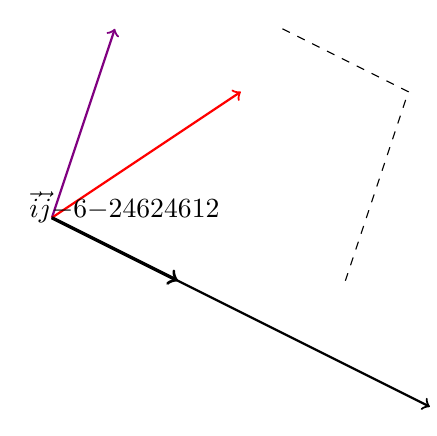
\begin{tikzpicture}[scale=.4]
\tkzInit[xmin=-3,xmax=13, ymin=-7, ymax=7]
\tkzRep[xlabel=$\vec{i}$, ylabel=$\vec{j}$]
\tkzDrawXY [noticks]%, label={}]


\draw [color=violet, thick, ->] (0,0) -- +(2,6) ; 
\draw [color=red, thick, ->] (0, 0 ) -- +(6, 4) ; 
\draw [color=black, very thick, ->] (0, 0 ) -- +(4, -2) ; 
\draw [color=black, thick, ->] (0, 0 ) -- +(12, -6) ; 

\tkzText(0,-6){\textcolor{black}{-}}\tkzLabelPoint[color=bistre,left](0, -6){$-6$}
\tkzText(0,-2){\textcolor{black}{-}}\tkzLabelPoint[color=bistre,left](0, -2){$-2$}
\tkzText(0,4){\textcolor{black}{-}} \tkzLabelPoint[color=bistre,left](0,4){$4$}
\tkzText(0, 6){\textcolor{black}{-}} \tkzLabelPoint[color=bistre, left](0, 6){$6$}



\tkzText(2,0){\textcolor{black}{|}} \tkzLabelPoint[color=bistre,below](2,0){$2$}
\tkzText(4,0){\textcolor{black}{|}} \tkzLabelPoint[color=bistre,below](4,0){$4$}
\tkzText(6,0){\textcolor{black}{|}} \tkzLabelPoint[color=bistre,below](6,0){$6$}
\tkzText(12,0){\textcolor{black}{|}} \tkzLabelPoint[color=bistre,below](12,0){$12$}

\draw[color=black, dashed] (2,6) -- (6, 4) -- (4, -2) ; 

\end{tikzpicture}

On a $\vec{u} + \vec{v}\left(\begin{array}{c} 6\\ 4 \end{array}\right)$ et $ 3 \vec{u}\left(\begin{array}{c} 12\\ -6 \end{array}\right)$
\newpage
\subsubsection{Démonstration} 

1. $\vec{u} + \overrightarrow{u'} = \left(x\vec{i} + y\vec{i}\right) + \left(x'\vec{i} + y'\vec{j}\right) $

$ \vec{u} + \overrightarrow{u'} = \left(x+x'\right) \vec{i} + \left(y + y'\right)\vec{j} $

$\lambda \vec{u} = \lambda \left(x\vec{i} + y\vec{j}\right)$

$\lambda \vec{u} = \lambda x\vec{i} + \lambda y\vec{j} $

\subsection{Vecteurs colinéaires}

Soit $\left(\vec{i}, \vec{j}\right)$.

\subsubsection{Notion de déterminant}

Soit $\vec{u}\left(\begin{array}{c} a\\ b \end{array}\right)$ et $\vec{v}\left(\begin{array}{c} c\\ d \end{array}\right)$

Par définition, on appelle le déterminant de $\vec{u}$ et de $\vec{v}$ : $\det\left(\vec{u}, \vec{v}\right) = \left| \begin{array}{cc}  a & c \\ b & d  \\ \end{array} \right| = ad- bc $

\subsubsection{Exemple \no 1}

Soient $\vec{u}\left(\begin{array}{c} 2\\ 1 \end{array}\right)$ et $\vec{v}\left(\begin{array}{c} 4\\ 5 \end{array}\right)$

$\det\left(\vec{u}, \vec{v}\right) = \left| \begin{array}{cc}  2 & 4 \\ 1 & 5  \\ \end{array} \right| = 10 - 4 = 6 $

\subsubsection{Exemple \no 2}

Soient $\vec{u}\left(\begin{array}{c} 8\\ -6 \end{array}\right)$ et $\vec{v}\left(\begin{array}{c} -4\\ 3 \end{array}\right)$

$\det\left(\vec{u}, \vec{v}\right) = \left| \begin{array}{cc}  8 & -4 \\ -6 & 3  \\ \end{array} \right| = 24 - 24 = 0 $

$\vec{v} = -\dfrac{1}{2} \vec{u} $

\subsubsection{Condition de colinéarité de deux vecteurs}

Soient $\vec{u} \neq \overrightarrow{0} $ et $ \vec{v} \neq \overrightarrow{0} $

$\vec{u}$ et $ \vec{v}$ sont colinéaires $\Longleftrightarrow det\left(\vec{u}, \vec{v}\right) = 0 $
\newpage 
\subsubsection{Démonstration}

\textbf{Sens gauche-droite}

Soient $\vec{u}$ et $ \vec{v}$ deux vecteurs colinéaires.

$\vec{u}\left(\begin{array}{c} a\\ b \end{array}\right)$ et $\vec{v}\left(\begin{array}{c} c\\ d \end{array}\right)$

Il existe $\lambda \in \R$ tel que $\vec{v} = \lambda \vec{u} $

On a alors : $\vec{u}\left(\begin{array}{c} a\\ b \end{array}\right)$ et $\vec{v}\left(\begin{array}{c} \lambda a\\ \lambda b \end{array}\right)$

$\det\left(\vec{u}, \vec{v}\right) = \left| \begin{array}{cc}  a & \lambda a \\ b & \lambda b  \\ \end{array} \right| = a \left(\lambda b\right) - b \left(\lambda a\right)= 0 $

\textbf{Sens droite-gauche}

Soient $\vec{u}$ et $\vec{v}$ deux vecteurs colinéaires tels que $\det(\vec{u}, \vec{v})=0$

$\vec{u}\left(\begin{array}{c} a\\ b \end{array}\right)$ et $\vec{v}\left(\begin{array}{c} c\\ d \end{array}\right)$ \\

L'un au moins des 2 nombres réels $a$ et $b$ n'est pas nul car $\vec{u} \neq \overrightarrow{0} $

Supposons par exemple $a \neq 0$ et posons $\lambda = \dfrac{c}{a}$ et $c = \lambda a$.

$\det (\vec{u}, \vec{v}) = 0$

$\left| \begin{array}{cc}  a & c \\ b & d  \\ \end{array} \right| = 10 - 4 = 6 $

$ad - bc = 0$

$ad - b\left(\lambda a \right) = 0 $

$ a \left( d - \lambda b\right) = 0 $ \\

\begin{tabular}{lll}
$ \underbrace{a = 0}_{\textrm{Impossible}}$ & ou & $d - \lambda b = 0$ \\
 & & $ d = \lambda b $ \\
  
\end{tabular}

Conclusion :

\begin{itemize}
\item $ c = \lambda a $
\item $ d = \lambda b$
\end{itemize}

Donc $\vec{v}\left(\begin{array}{c} \lambda a\\ \lambda b \end{array}\right)$, et $\vec{v}$ est colinéaire à $\vec{u}$.
\newpage
\subsection{Exercices}

\subsubsection{Exercice \no 1}

Soit ABC un triangle.

Soit A' le milieu de $\left[BC\right]$

Soit G le centre de gravité de ABC.

On se place dans le repère $\left(A, \overrightarrow{AB}, \overrightarrow{AC}\right)$

Déterminer les coordonnées de A' dans $\left(A, \overrightarrow{AB}, \overrightarrow{AC}\right)$, puis les coordonnées de G dans $\left(A, \overrightarrow{AB}, \overrightarrow{AC}\right)$.\\

% exercice 1
\begin{tikzpicture}[scale=0.4]
\coordinate (G) at (0.2,-0.07) ; 

\draw (6,8) node [above] {$A$} --  (-8.7,-5) node [left] {$B$} -- (8.7,-5) node [right] {$C$}-- (6, 8) ; 
\draw [dashed] (6,8) -- (0,-5) node [below] {$A'$} ;
\draw [dashed](-8.7,-5) -- (7.4,1.5) node [right] {$B'$} ;
\draw [dashed](8.7,-5) -- (-1.3,1.5) node [left] {$C'$} ;
\draw (2,-0.7) node [below right] {$G$} ; 

\end{tikzpicture}\\

$\overrightarrow{AA'} = \dfrac{1}{2} \overrightarrow{AB} + \dfrac{1}{2}\overrightarrow{AC}$\\

Donc $A'\left(\dfrac{1}{2}, \dfrac{1}{2}\right)$\\

$\overrightarrow{AG} = \dfrac{1}{3} \overrightarrow{AB} + \dfrac{1}{3}\overrightarrow{AC}$\\

Donc $G\left(\dfrac{1}{3}, \dfrac{1}{3}\right)$\\

\textbf{Remarque}\\

$A\left(0,0\right) \textrm{car} \overrightarrow{AA} = 0\overrightarrow{AB} + 0\overrightarrow{AC}$\\

$B\left(1,0\right) \textrm{car} \overrightarrow{AB} = 1\overrightarrow{AB} + 0\overrightarrow{AC}$\\

$C\left(0,1\right) \textrm{car} \overrightarrow{AC} = 0\overrightarrow{AB} + 1\overrightarrow{AC}$\\

\newpage
\subsubsection{Exercice \no 2}

Soit $\left(O,\vec{i}, \vec{j}\right)$ un repère. 

Soient les points $A\left(4,2\right)$, $B\left(-4,-4\right)$, $C\left(2,-8\right)$, $D\left(10,-2\right)$.


1.  Montrer par 2 méthodes que ABCD est un parallélogramme.

\vspace*{-9cm}
\begin{tikzpicture}[scale=.6]
\tkzInit[xmin=-5,xmax=12, ymin=-9, ymax=4]
\tkzDrawXY [color=black, noticks] 
\tkzRep[xlabel=$\vec{i}$, ylabel=$\vec{j}$]
\tkzLabelPoint[color=bistre,below left](0,0){$0$}

\tkzDefPoint (4,2){A} \tkzDefPoint (-4, -4){B} \tkzDefPoint (2, -8){C}
\tkzDefPoint (10, -2){D} \tkzDefPoint (3,-3){I}

\draw [color=black, thick] (A) node [above] {$A$}-- 
(B) node [below] {$B$} -- (C) node [below right] {$C$}-- (D) node [below right] {$D$} -- cycle ;   

\draw[color=black] (A) -- (C);  
\draw[color=black] (B) -- (D) ;

\tkzLabelPoint[color=black, below left](I){$I$}

\tkzText(-4,0){\textcolor{bistre}{|}} \tkzLabelPoint[color=bistre, below](-4,0){$-4$}
\tkzText(4,0){\textcolor{bistre}{|}} \tkzLabelPoint[color=bistre, below](4,0){$4$}
\tkzText(10,0){\textcolor{bistre}{|}} \tkzLabelPoint[color=bistre, below](10,0){$10$}
\tkzText(0,-8){\textcolor{bistre}{-}} \tkzLabelPoint[color=bistre, right](0,-8){$-8$}
\tkzText(0, -4){\textcolor{bistre}{-}}  \tkzLabelPoint[color=bistre, left](0,-4){$-4$}
\tkzText(0, -2){\textcolor{bistre}{-}}  \tkzLabelPoint[color=bistre, left](0,-2){$-2$}
\tkzText(0, 22){\textcolor{bistre}{-}}  \tkzLabelPoint[color=bistre, left](0,2){$2$}
\end{tikzpicture}\\

\textbf{Première méthode} \\

$x_B - x_A = -4 - 4 = -8 $

$y_B - y_A = -4 - 2 = -6 $

Donc $\overrightarrow{AB}\left(\begin{array}{c} -8\\ -6 \end{array}\right)$ \\

$x_C - x_D = 2 - 10 = -8 $

$ y_C - y_D = -8 - \left(-2\right) = -6 $

Donc $\overrightarrow{DC}\left(\begin{array}{c} -8\\ -6 \end{array}\right)$ 

On a $\overrightarrow{AB} = \overrightarrow{DC}$ donc ABCD est un parallélogramme. \\

\textbf{Deuxième méthode}\\

Soit I le milieu de $\left(AC\right)$ : \\

\begin{itemize}
\item[*] $x_I = \dfrac{x_A + x_C}{2} = \dfrac{4+2}{2} = 3 $\\
\item[*] $ y_I = \dfrac{y_A + y_C}{2} = \dfrac{2 - 8}{2} = -3 $\\
\end{itemize}

Donc $I\left(3,-3\right)$ \\

Soit J le milieu de $\left(BD\right)$ : \\

\begin{itemize}
\item $x_J = \dfrac{x_B + x_D}{2} = \dfrac{-4+10}{2} = 3 $\\
\item $ y_J = \dfrac{y_B + y_D}{2} = \dfrac{-4 -2}{2} = -3 $\\
\end{itemize}

Donc $J\left(3,-3\right)$\\

$I = J$, donc ABCD est un parallélogramme.  \\

2. Soient $A\left(-6,0\right)$, $ B\left(-1,3\right)$, $C\left(7,-5\right)$, et $D\left(x,y\right)$

Déterminer x et y pour que ABCD soit un parallélogramme. (2 méthodes) \\

% Première méthode
\begin{tikzpicture}[scale=.5]

\tkzInit[xmin=-7,xmax=8, ymin=-9, ymax=4]
\tkzRep[xlabel=$\vec{i}$, ylabel=$\vec{j}$]
\tkzDrawXY [color=black, noticks]%, label={}]
\tkzLabelPoint[color=bistre,below left](0,0){$0$}

\draw [color=black]  (-6, 0) node [above] {$A$} -- (-1, 3) node [above] {$B$} -- (7, -5) node [right] {$C$} -- (2, -8) node [below] {$D$} -- cycle  ; 
\draw [color=black] (-6,0) -- (.5, -2.5) node [above] {$I$} -- (7, -5) ; 
\tkzDrawPoint[color=black](.5,-2.5) 
\tkzLabelPoint[color=bistre, below left](-6,0){$-6$}
\tkzText(-1,0){\textcolor{bistre}{|}} \tkzLabelPoint[color=bistre, below left](-1,0){$-1$}
\tkzText(7,0){\textcolor{bistre}{|}} \tkzLabelPoint[color=bistre, below left](7,0){$7$}
\tkzText(0,-5){\textcolor{bistre}{-}} \tkzLabelPoint[color=bistre, left](0,-5){$-5$}
\tkzText(0, 3){\textcolor{bistre}{-}}  \tkzLabelPoint[color=bistre, left](0,3){$3$}

\end{tikzpicture}

$D\left(2,-8\right)$ On conjecture que $D\left(2,-8\right)$.\\

\textbf{Première méthode}\\

$x_B - x_A = -1 -\left(-6\right) = 5 $

$ y_B - y_A = 3 - 0 = 3 $\\

Donc $\overrightarrow{AB}\left(\begin{array}{c} 5\\ 3 \end{array}\right)$

$x_C - x_D = 7 - x$

$ y_C - y_D = -5 - y $ \\


Donc $\overrightarrow{DC}\left(\begin{array}{c} 7-x\\ -5-y \end{array}\right)$


\begin{tabular}{lll}
$ABCD$ est un parallélogramme & $\Longleftrightarrow$ & $\overrightarrow{AB} = \overrightarrow{DC} $ \\
& $\Longleftrightarrow$ & $ \begin{cases} 7 - x = 5 \\ -5 - y = 3 \end{cases}$ \\
& $ \Longleftrightarrow$ & $ \begin{cases} -x = -2 \\ -y = 8 \end{cases} $ \\
& $\Longleftrightarrow$ & $ \begin{cases}x = 2 \\ y = -8 \end{cases} $ \\
\end{tabular}

Donc $D\left(2,-8\right)$\\

\textbf{Deuxième méthode}\\
Soient I le milieu de $ \left[AC\right] $ et J le milieu de $\left[BD\right]$.\\

$x_I = \dfrac{-6 + 7}{2} = \dfrac{1}{2} $\\

$ y_I = \dfrac{0-5}{2} = -\dfrac{5}{2} $\\

$ x_J = \dfrac{-1 + x}{2} $\\

$ y_J = \dfrac{3 + y}{2} $\\

\begin{tabular}{lll}
$ABCD$ est un parallélogramme & $\Longleftrightarrow$ & I = J \\
& $\Longleftrightarrow$ & $ \begin{cases} \dfrac{-1 + x}{2} = \dfrac{1}{2} \\ 
              \\
\dfrac{3 + y}{2} = -\dfrac{5}{2} \end{cases}$ \\
&& \\
& $ \Longleftrightarrow$ & $ \begin{cases} -1 + x = 1 \\ 3 + y = -5 \end{cases} $ \\
&& \\
& $\Longleftrightarrow$ & $ \begin{cases} x = 2 \\ y = -8 \end{cases} $ \\
\end{tabular}


\newpage
\subsubsection{Exercice \no 3}

Soit $\left(O, \vec{i}, \vec{j}\right)$ un repère. \\

1. Soient $A\left(5,3\right)$, $B\left(8,5\right)$, $C\left(13,9\right)$.

Les points A, B et C sont-il alignés ?

% Exercice n°3
\begin{tikzpicture}[scale=.6]

\tkzInit[xmin=-2,xmax=15, ymin=-2, ymax=9]
\tkzDrawXY [color=black, noticks] 
\tkzLabelPoint[color=bistre,below left](0,0){$0$}
 
\draw [color=black] (-1,-1) -- (14,9) ; 
\tkzDrawPoint[color=black](5,3) \tkzLabelPoint[color=black, above](5,3){$A$} 
\tkzDrawPoint[color=black](8, 5) \tkzLabelPoint[color=black, above](8,5){$B$}
\tkzDrawPoint[color=black](13,8) \tkzLabelPoint[color=black, below](13,8){$C$}  

\tkzText(5,0){\textcolor{bistre}{|}} \tkzLabelPoint[color=bistre, below](5,0){$5$}
\tkzText(8,0){\textcolor{bistre}{|}} \tkzLabelPoint[color=bistre, below](8,0){$8$}
\tkzText(13,0){\textcolor{bistre}{|}} \tkzLabelPoint[color=bistre, below](13,0){$13$}
\tkzText(0,3){\textcolor{bistre}{-}} \tkzLabelPoint[color=bistre, left](0,3){$3$}
\tkzText(0, 5){\textcolor{bistre}{-}}  \tkzLabelPoint[color=bistre, left](0,5){$5$}
\tkzText(0, 8){\textcolor{bistre}{-}}  \tkzLabelPoint[color=bistre, left](0,8){$8$}

\end{tikzpicture}

$x_B - x_A = 8 - 5 = 3 $

$ y_B - y_A = 5 - 3 = 2 $

Donc $\overrightarrow{AB}\left(\begin{array}{c} 3\\ 2 \end{array}\right)$ \\

$ x_C - x_A = 13 - 5 = 8 $

$ y_C - x_A = 8 - 3 = 5 $

Donc $\overrightarrow{AC}\left(\begin{array}{c} 8\\ 5 \end{array}\right)$

$\det\left(\overrightarrow{AB}, \overrightarrow{AC}\right) = \left| \begin{array}{cc}  3 & 8 \\ 2 & 5  \\ \end{array} \right| = 15- 16 = -1 $

$\det\left(\overrightarrow{AB}, \overrightarrow{AC}\right) \neq 0 $

$\overrightarrow{AB}$ et $ \overrightarrow{AC}$ ne sont pas colinéaires. Donc les points A, B et C ne sont pas alignés. \\

\newpage

2. Soient $A\left(-4,5\right)$, $B\left(4,1\right)$, $C\left(x,-1\right)$.

Déterminer $x$ pour que les points A, B et C soient alignés.

$\overrightarrow{AB}\left(\begin{array}{c} 8\\ -4 \end{array}\right)$ et $\overrightarrow{AC}\left(\begin{array}{c} x+4\\ -6 \end{array}\right)$

\begin{tabular}{lll}
A, B et C sont alignés & $\Longleftrightarrow $ & $\overrightarrow{AB}$ et $\overrightarrow{AC}$ sont colinéaires. \\
& $\Longleftrightarrow$ & $\det\left(\overrightarrow{AB}, \overrightarrow{AC} \right) = 0 $ \\
& $\Longleftrightarrow$ & $-48 + 4\left(x+4\right) = 0$ \\
& $\Longleftrightarrow$ & $4\left(x+4\right) = 48 $ \\
& $ \Longleftrightarrow$ & $4x + 16 = 48$ \\
& $ \Longleftrightarrow$ & $4x = 32$ \\
& $\Longleftrightarrow $ & $x = 8 $ \\
\end{tabular}

Donc $C\left(8, -1\right)$

% Exercice n°3 suite .
\begin{tikzpicture}[scale=.6]

\tkzInit[xmin=-7,xmax=13, ymin=-4, ymax=6]
\tkzDrawXY [color=black, noticks] 
\tkzLabelPoint[color=bistre,below left](0,0){$0$}
 
\draw [color=black] (-6,6) -- (12,-3) ; 
\tkzDrawPoint[color=black](-4,5) \tkzLabelPoint[color=black, above](-4,5){$A$} 
\tkzDrawPoint[color=black](4, 1) \tkzLabelPoint[color=black, above](4,1){$B$}
\tkzDrawPoint[color=black](8,-1) \tkzLabelPoint[color=black, below](8,-1){$C$}  

\tkzText(-4,0){\textcolor{bistre}{|}} \tkzLabelPoint[color=bistre, below](-4,0){$-4$}
\tkzText(4,0){\textcolor{bistre}{|}} \tkzLabelPoint[color=bistre, below](4,0){$4$}
\tkzText(8,0){\textcolor{bistre}{|}} \tkzLabelPoint[color=bistre, below](8,0){$8$}
\tkzText(0,-1){\textcolor{bistre}{-}} \tkzLabelPoint[color=bistre, left](0,-1){$-1$}
\tkzText(0, 1){\textcolor{bistre}{-}}  \tkzLabelPoint[color=bistre, left](0,1){$1$}
\tkzText(0, 5){\textcolor{bistre}{-}}  \tkzLabelPoint[color=bistre, left](0,5){$5$}
\end{tikzpicture}

\newpage 
\subsubsection{Exercice \no 4}

Soit $\left(O, \vec{i}, \vec{j}\right)$ un repère.

Soient $A\left(-7,12\right)$, $B\left(-1,-8\right)$, $C\left(12,-5\right)$ et $D\left(4,1\right)$.

1. Déterminer les coordonnées de I défini par $ \overrightarrow{IA} + \overrightarrow{IB} + \overrightarrow{IC} + \overrightarrow{ID} = \overrightarrow{0} $

2. Déterminer les coordonnées de G, centre de gravité du triangle BCD. Montrer que les points A, G et I sont alignés.

3. Déterminer les coordonnées du point $G_1$, milieu de $\left[AB\right]$, puis ceux de $G_2$, milieu de $\left[CD\right]$. Montrer que I est le milieu de $\left[G_1G_2\right]$.

% Exercice n°4 
\begin{tikzpicture}[scale=.8]

\tkzInit[xmin=-9,xmax=13, ymin=-9, ymax=13]
\tkzDrawXY [color=black, thick, ticks] 
\tkzRep[xlabel=$\vec{i}$, ylabel=$\vec{j}$]
\tkzLabelPoint[color=bistre,below left](0,0){$0$}
% \tkzGrid

\tkzDefPoint (-7, 12){A} \tkzDefPoint (-1, -8){B} \tkzDefPoint (12, -5){C}
\tkzDefPoint (4, 1){D} \tkzDefPoint (-4, 2){G1} \tkzDefPoint (8, -2){G2}  
\tkzDefPoint (2, 0){I} \tkzDefPoint (5, -4){G}  
\draw [color=black, thick] (A) node [above] {$A$} --
(B) node [below] {$B$} -- (C) node [below right] {$C$} -- 
(D) node [right] {$D$} -- cycle ;   

\draw[color=black, dashed] (A) -- (G) node [right] {$G$} ;  
\draw[color=black, dashed] (B) -- (D) node [right] {$D$} ;
\draw[color=black, dashed] (G1) node [left] {$G_{1}$} -- (G2) node [below] {$G_{2}$};

\tkzLabelPoint[color=bistre, below left](I){$I$}

\tkzText(-7,0){\textcolor{bistre}{|}} \tkzLabelPoint[color=bistre, below](-7,0){$-7$}
\tkzText(-1,0){\textcolor{bistre}{|}} \tkzLabelPoint[color=bistre, below](-1,0){$-1$}
\tkzText(12,0){\textcolor{bistre}{|}} \tkzLabelPoint[color=bistre, below](12,0){$12$}
\tkzText(0,-8){\textcolor{bistre}{-}} \tkzLabelPoint[color=bistre, right](0,-8){$-8$}
\tkzText(0, -5){\textcolor{bistre}{-}}  \tkzLabelPoint[color=bistre, left](0,-5){$-5$}
\tkzText(0, 12){\textcolor{bistre}{-}}  \tkzLabelPoint[color=bistre, left](0,12){$12$}
\end{tikzpicture}

\newpage
\vspace*{-1.5cm}
On a $I\left(x,y\right)$.

$\overrightarrow{IA}\left(\begin{array}{c} -7 - x\\ 12 - y \end{array}\right)$ \\

$\overrightarrow{IB}\left(\begin{array}{c} -1 - x\\ -8 - y \end{array}\right)$ \\

$\overrightarrow{IC}\left(\begin{array}{c} 12 - x\\ -5 - y \end{array}\right)$ \\

$\overrightarrow{ID}\left(\begin{array}{c} 4 - x\\ 1 - y \end{array}\right)$ \\

$ \overrightarrow{IA} + \overrightarrow{IB} + \overrightarrow{IC} + \overrightarrow{ID} \left(\begin{array}{c} 8 - 4x\\ -4y \end{array}\right)$ \\

\begin{tabular}{lll}
$\overrightarrow{IA} + \overrightarrow{IB} + \overrightarrow{IC} + \overrightarrow{ID} = \overrightarrow{0}$ & $\Longleftrightarrow$&  $ \begin{cases} 8 - 4x = 0 \\ -4y = 0 \end{cases}$ \\
& $\Longleftrightarrow$ & $\begin{cases}-4x = -8 \\ y + 0 \end{cases}$ \\
& $\Longleftrightarrow$ & $\begin{cases} x = 2 \\ y = 0 \end{cases}$ \\
\end{tabular}

Donc $I\left(2,0\right)$.\\

2. $G\left(\dfrac{x_B + x_C + x_D}{3} ; \dfrac{y_B + y_C + y_D}{3}\right)$\\

$ G\left(\dfrac{-1 + 12+ 4}{3} ; \dfrac{-8 - 5 + 1}{3}\right)$\\

$ G \left(5,-4\right) $\\

On a $\overrightarrow{AI}\left(\begin{array}{c} 9\\ -12 \end{array}\right)$ et $\overrightarrow{AG}\left(\begin{array}{c} 12\\ -16 \end{array}\right)$\\

$\det\left(\overrightarrow{AI}, \overrightarrow{AG}\right) = \left| \begin{array}{cc}  9 & 12 \\ -12 & -16  \\ \end{array} \right| = - 144 - \left(-140\right) = 0 $\\

Donc $\overrightarrow{AI}$ et $\overrightarrow{AG}$ sont colinéaires.

Donc les points A, I et G sont alignés.\\

3. $G_1 \left(\dfrac{-7 - 1}{2} , \dfrac{12-4}{2}\right)$\\

$ G_1 \left(-4, 2\right) $\\

$ G_2 \left(\dfrac{12 + 4}{2} , \dfrac{-5 + 1}{2} \right) $\\

$ G_2\left(8,-2\right) $\\

Soit J le milieu de $\left[G_1G_2\right]$\\

On a $J\left(\dfrac{-4 + 8}{2}, \dfrac{2-2}{2} \right)$\\

$J\left(2,0\right)$  

I = J.

Donc I est l milieu de $\left[G_1G_2\right]$.
\newpage

\subsubsection{Exercice \no 5}

Soit $\left(\vec{i}, \vec{j}\right)$ une base.

Soit $m \in \R$

Soient $\vec{u}\left(\begin{array}{c} m+7\\ -10 \end{array}\right)$, $\vec{v}\left(\begin{array}{c} m-47\\ 50 \end{array}\right)$ et $\overrightarrow{w}\left(\begin{array}{c} m+3\\ m-6 \end{array}\right)$

1. Déterminer m pour que $\vec{u}$ et $\vec{v}$ soient colinéaires. Exprimer alors $\vec{u}$ en fonction de $\vec{v}$.\\

2. Déterminer m pour que $\vec{u}$ et $\overrightarrow{w}$ soient colinéaires. Exprimer alors $\overrightarrow{w}$ en fonction de $\vec{u}$.\\


\begin{tabular}{lll}
$\vec{u}$ et $\vec{v}$ sont colinéaires & $\Longleftrightarrow$ & $\det\left(\vec{u}, \vec{v}\right) = 0$ \\
& $\Longleftrightarrow$ & $ 50\left(m+7\right) + 10 \left(m - 47\right) = 0$ \\
& $\Longleftrightarrow$ & $ 50m + 350 + 10m - 470 = 0 $ \\
& $\Longleftrightarrow$ & $ 60m - 120 = 0 $ \\
& $\Longleftrightarrow$ & $ 60 = 120 $ \\
& $\Longleftrightarrow$ & $ m = 2 $ \\
\end{tabular}

$\det\left(\vec{u}, \vec{v}\right) = \left| \begin{array}{cc}  9 & -45 \\ -10 & 50  \\ \end{array} \right| = 450 - 450 = 0 $

$\vec{u}\left(\begin{array}{c} 9\\ -10 \end{array}\right)$ et $\vec{v}\left(\begin{array}{c} -45\\ 50 \end{array}\right)$.

Donc $\vec{v} = -5\vec{u} $.\\

\begin{tabular}{lll}
$\vec{u}$ et $\overrightarrow{w}$ sont colinéaires & $\Longleftrightarrow$ & $\det\left(\vec{u}, \overrightarrow{w}\right) = 0$ \\
& $\Longleftrightarrow$ & $\left(m+7\right)\left(m-6\right) + 10 \left(m+3\right) = 0 $ \\
& $\Longleftrightarrow$ & $m^2 - 6m + 7m - 42 + 10m + 30 = 0 $\\
& $\Longleftrightarrow$ & $ m^2 +11m -12 = 0 $ \\
& $\Longleftrightarrow$ & $ \left(m^2 + 11m + \dfrac{121}{4} \right) - \dfrac{169}{4} = 0 $ \\
& $\Longleftrightarrow$ & $ \left(m+\dfrac{11}{2} \right)^2 - \left(\dfrac{13}{2} \right)^2 = 0 $ \\
& $\Longleftrightarrow$ & $ \left(m + \dfrac{11}{2} - \dfrac{13}{2} \right) \left(m + \dfrac{11}{2} + \dfrac{13}{2}\right) = 0 $ \\
& $\Longleftrightarrow$ & $ \left(m-1\right)\left(m + 12\right) = 0 $ \\
\end{tabular}

\begin{tabular}{lll}
$ m-1 = 0$ & ou & $m+12 = 0$ \\
$m = 1$ & ou & $ m = -12 $ \\
\end{tabular}\\

\textbf{Premier cas}

On a $\vec{u}\left(\begin{array}{c} 8\\ -10 \end{array}\right)$ et $\overrightarrow{w}\left(\begin{array}{c} 4\\ -5 \end{array}\right)$, donc $\overrightarrow{w} = \dfrac{1}{2} \vec{u}$.\\

\textbf{Deuxième cas}

On a $\vec{u}\left(\begin{array}{c} -5\\ -10 \end{array}\right)$ et $\overrightarrow{w}\left(\begin{array}{c} -9\\ -18 \end{array}\right)$, donc $\overrightarrow{w} = \dfrac{9}{5} \vec{u}$.


\ifdefined\COMPLETE
\else
    \end{document}
\fi